% - How to build the CRT
\section{The Cosmic Ray Tracker Front-End Board}
The Front-End Board \gls{feb} is designed to serve a \gls{crt} panel and process its signals to event data.
The \gls{feb} is illustrated in figure \ref{fig:feb}.
This section aims to explain the \gls{feb}'s functionalities and list some of its features.
For more detailed information please refer to the \gls{feb}'s technical description\cite{Auger:2016vpo}.

\subsection{The Front-End Board in a nutshell}
The \gls{feb} completes a \gls{crt} module by supplying the \glspl{sipm} with a bias voltage and read out their signals.
The \gls{feb} features a configurable bias voltage and threshold as well as a triggering logic to reduce background signal.
The bias voltage is used to tune the gain of every \gls{sipm} while the threshold is used to discriminate events below a certain signal.
Several \glspl{feb} can be set in coincidence, triggering events only if all the \glspl{feb} put in coincidence trigger an event in a short time window.
This allows to arrange more complex setups.
When several \glspl{feb} are used, they can be daisy-chained to send data via network to a single host.

\begin{figure}
  \centering
  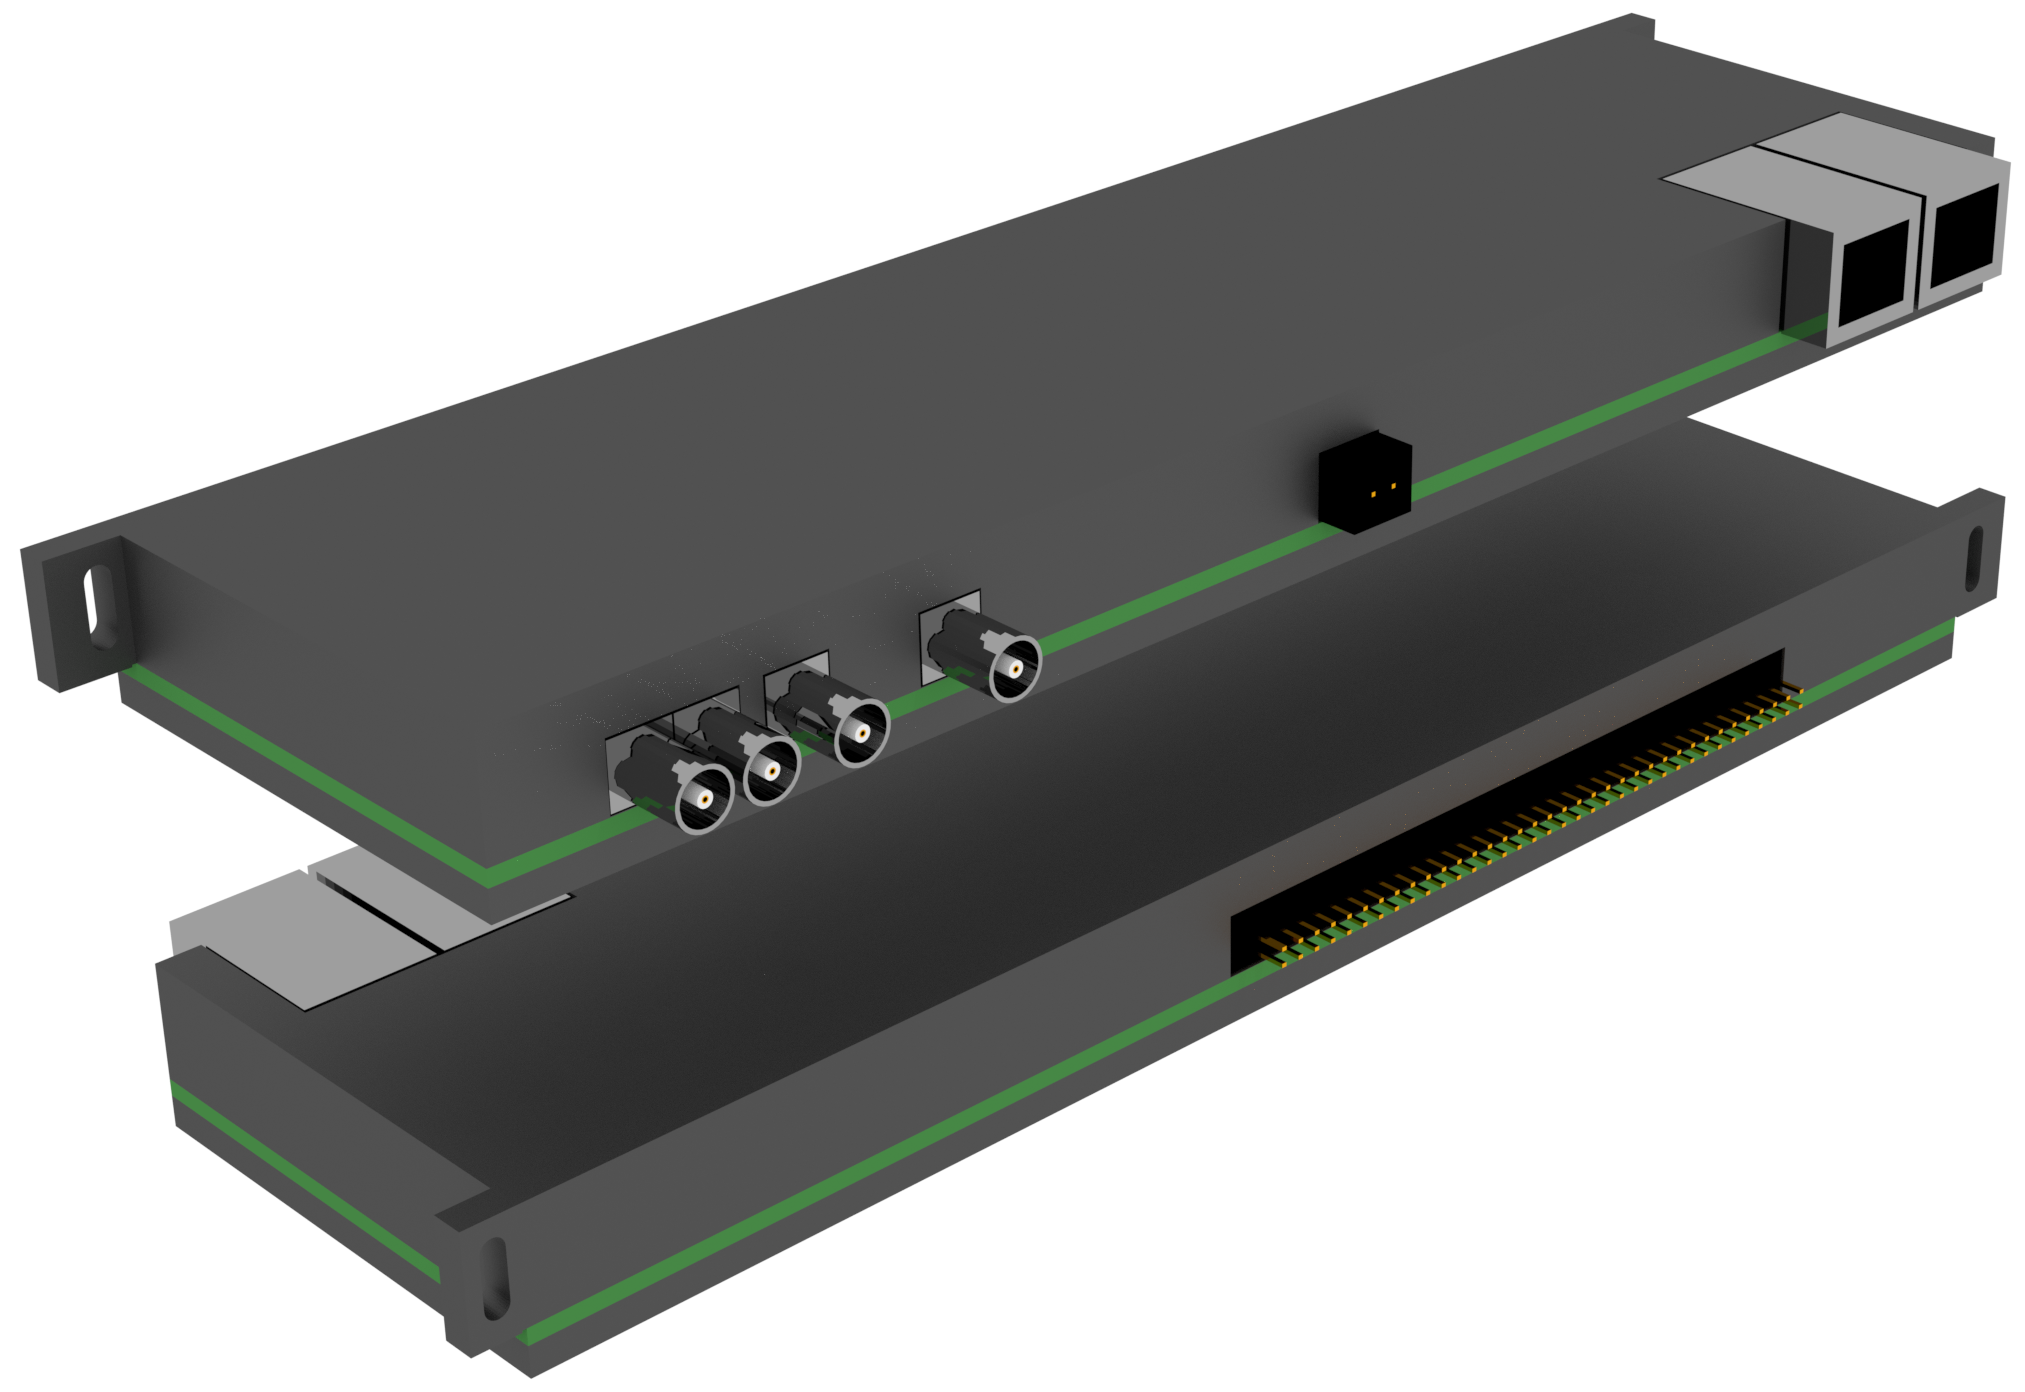
\includegraphics[width=\textwidth]{FEB}
  \caption{%
    This figure shows the ports of the \gls{feb} (top) and the connector for the \gls{crt} panel (bottom).
    The ports are (fltr): TIN, TOUT for external coincidence signals, T2, T1 for time reference signals, power connector, 2x fast ethernet.
    The electronic components' board is visible from outside (green).
  }
  \label{fig:feb}
\end{figure}

\subsection{Bias voltage generator}
Bias voltage is given by two opposed voltages: A stabilized power supply and the voltage output of a \gls{dac}.
The voltage of the power supply is adjustable in a range from 50V to 90V by varying manually a trimmer resistor and is common for all 32 \glspl{sipm} served by the \gls{feb}.
Individual adjustments for every channel are made using the output the \gls{dac} supplied on board.
See figure \ref{fig:voltage_generator} for a simplified scheme of the electronic circuit.

\begin{figure}
  \centering
  \begin{circuitikz}
    \node[ground] (g1) at (0, -1) {};
    \node[ground] (g2) at (8, -1) {};
    
    \draw (0, -1) -- (0, 0) to[V=$V_\text{DAC}$] (2, 0) to[R, -*] (4, 0) to[D] (6, 0);
    \draw (8, -1) -- (8, 0) to[V=$V_\text{trimmed}$] (6, 0);
    \draw (4, 0) to[short, -o] (4, -2);
    \draw (4, -2) node[right] {$S_i$};
  \end{circuitikz}
  \caption{%
    The bias voltage is generated using a voltage source trimmed by a resistor.
    Voltage fine tuning for every channel is made with a configurable \gls{dac}'s output.
    The \gls{dac}'s constant output corresponds to a DC-offset of the signal lines, the \gls{dac}'s full range is from +0.5V to +4.5V.
    Since the \gls{dac}'s output is positive, increasing its value actually reduces the effective bias voltage for the \gls{sipm}.
    The \gls{sipm} is depicted as a single diode in this scheme for simplicity.
  }
  \label{fig:voltage_generator}
\end{figure}

\subsection{Triggering logic}
One of the \gls{feb}'s features is to trigger events only when both \glspl{sipm} of the same scintillating bar present simultaneously a sufficently high signal.
The signal $S_i$ -- for the $i$th \gls{sipm} -- is amplified a charge amplifier and shaped with a RC-CR-shaper.
If the shaped signal is greater than the set threshold, the output of the discriminator $T_i$ is positive.
This output is combined with the corresponding signal of the associated \gls{sipm}, generating the pair trigger signal $P_i$.
If one of the pairs trigger a signals is positive, the \gls{cpu} tarts digitazion of the event.
\marginnote{This coincidence requirement reduces the number of events caused by incident gamma radiation significantly.}
Amplification, shaping and discrimination is done by CITIROC ASIC and signal logic is processed by a SPARTAN-6 \gls{fpga}.
See figure \ref{fig:fast_shaper_discriminator} for an illustration of the electronic circuit.

\begin{figure}
  \centering
  \begin{circuitikz}

    \node[buffer]     (amp1)    at (0, 0) {};
    \node[coordinate] (c1)      at (2, 0) {};
    \node[coordinate] (c2)      at (4, 0) {};
    \node[coordinate] (c2t)     at (4, 1.5) {};
    \node[coordinate] (c2tt)    at (4, 3) {};
    \node[buffer]     (amp2)    at (5, 0) {};
    \node[coordinate] (c3b)     at (6, -1) {};
    \node[ground]     (ground)  at (6, -2.5) {};
    \node[coordinate] (c3)      at (6, 0) {};
    \node[coordinate] (c3t)     at (6, 1.5) {};
    \node[coordinate] (c3tt)    at (6, 3) {};

    \node[op amp, yscale=-1]  (amp) at (8, -0.5) {};
    \node[and port]   (and) at (12, -0.775) {};

    % Inputs
    \draw (-1, 0) node[left] {$S_{2i}$};
    \draw (-1, 0) to[short, o-] (amp1.in);

    % RC-CR shaper
    \draw (amp1.out) to[R] (c1) to[C, -*] (c2);
    \draw (c2) -- (c2t) to[R, *-*] (c3t) -- (c3);
    \draw (c2) -- (c2tt) to[C] (c3tt) to[short, -*] (c3);
    \draw (c2) -- (amp2.in);
    \draw (amp2.out) -- (amp.+);

    % Connections to discriminator
    \draw (ground) to[V=$V_\text{DAC}$] (c3b) -- (amp.-);

    % Connections to the and port
    \draw (amp.out) -- (and.in 1);
    \draw (and.out) to[short, -o] (and.out);

    % Labels
    \draw (and.out)  node[right] {$P_i$};
    \draw (and.in 2) node[left] {$T_{2i+1}$};
    \draw (and.in 2) to[short, o-] (and.in 2);
    \draw (and.in 1) node[above left] {$T_{2i}$};

  \end{circuitikz}
  \caption{%
    Scheme of the electronic circuit to generate the trigger signal for a pair $P_i$ from the signals of two \glspl{sipm} $S_{2i}$ and $S_{2i+1}$.
    The amplifier, shaper and discriminator to generate associated signal $T_{2i+1}$ are not displayed for simplicity.
  }
  \label{fig:fast_shaper_discriminator}
\end{figure}

\subsection{Analog signal readout and digitization}
The \gls{feb} starts signal readout when an event trigger signal is triggered.
In that case the signal of the \glspl{sipm} is amplified, shaped using a slow RC-CR shaper and stored in a sample-and-hold circuit.
The stored analog signals are then digitized one by one using a 12-bit \gls{adc} and an analog multiplexer, to switch between the signals to digitalize.
Figure \ref{fig:slow_shaper} illustrates the electronic circuit.

\begin{figure}
  \centering
  \begin{circuitikz}

    \node[buffer] (amp1) at (0, 0) {};
    \node[coordinate] (c1) at (2, 0) {};
    \node[coordinate] (c2) at (4, 0) {};
    \node[coordinate] (c2t) at (4, 1.5) {};
    \node[coordinate] (c2tt) at (4, 3) {};
    \node[buffer] (amp2) at (5, 0) {};
    \node[coordinate] (c3) at (6, 0) {};
    \node[coordinate] (c3t) at (6, 1.5) {};
    \node[coordinate] (c3tt) at (6, 3) {};

    % Inputs
    \draw (-1, 0) node[left] {$S_i$};
    \draw (-1, 0) to[short, o-] (amp1.in);

    % RC-CR shaper
    \draw (amp1.out) to[R] (c1) to[C, -*] (c2);
    \draw (c2) -- (c2t) to[R, *-*] (c3t) -- (c3);
    \draw (c2) -- (c2tt) to[C] (c3tt) to[short, -*] (c3);
    \draw (c2) -- (amp2.in);
    \draw (amp2.out) -- (c3) -- ($(amp2.out) + (1, 0)$);
    \draw ($(amp2.out) + (1, 0)$) node[above] {$I_i$};

    % Switch and ADC
    \draw ($(amp2.out) + (1, 0)$)
      to[generic, l=S\&H] ($(amp2.out) + (3, 0)$)
      to[ospst=MUX] ($(amp2.out) + (4, 0)$)
      to[generic, l=ADC, -o] ($(amp2.out) + (6, 0)$);

  \end{circuitikz}
  \caption{%
    A series of amplificators and RC-CR slow shapers are used to treat the diode's signal before beind stored in the hold circuit.
  }
  \label{fig:slow_shaper}
\end{figure}

\subsection{Event data structure \& storage}
When an event is striggered and as soon as the \gls{adc} process is completed for all 32 channels, the result is combined with the time stamp to a packet of the following structure:

\begin{minted}{c}
  typedef struct {
    uint32_t flags;
    uint32_t T1;
    uint32_t T2;
    uint16_t adc[32];
  } FEBEVT_t;
\end{minted}

These event packets are stored in the internal ring buffer.
Once the capacity of 1024 events is reached, new events will override present ones.
The number of overwritten events is passed in the flags of the event packet.

\subsection{The Front-End Board software}

\paragraph{febdrv} communicates with \gls{feb} and sends commands to it.
febdrv allows to switch bias, data adquisition and configure the \gls{feb}.
It also publishes statistics and stati of the connected \glspl{feb} and their observed event packets.

\paragraph{febctl} sends commands to the febdrv to start and stop \gls{daq} and switch the \gls{feb}'s bias voltage.

\paragraph{febconf} reads configurations from files and sends them to the febdrv to change the \gls{feb}'s settings.

\paragraph{febmon} displays current status of the \gls{feb} published by febdrv.


